\subsection{Kernel Treiber}
\subsubsection{Temperatursensor über \acrshort{i2c}}

\Gls{i2c} Adapter Initialisieren.
\begin{lstlisting}[language=C]
test_i2c_adapter = i2c_get_adapter(I2C_BUS_AVAILABLE);
if(test_i2c_adapter == NULL)	{
    printk(KERN_CRIT "Fanctrl: No I2C Adapter found");
}	else	{
    printk(KERN_DEBUG "Fanctrl: Found I2C Adapter");
    test_i2c_client = i2c_new_client_device(test_i2c_adapter, &test_i2c_board_info);
    i2c_add_driver(&test_driver);
    i2c_put_adapter(test_i2c_adapter);
}
\end{lstlisting}

\Gls{i2c} Adapter De-initialisieren.
\begin{lstlisting}[language=C]
if(test_i2c_client != NULL)	{
    i2c_unregister_device(test_i2c_client);
    i2c_del_driver(&test_driver);
}
\end{lstlisting}

Der \texttt{TMP102} Sensor gibt Messdaten mit 13-Bit Präzision bei einer Auflösung von $0.0625\si{\degree C}$ am \gls{lsb}.
Um einen Messwert zu einer Temperatur zu konvertieren müssen zuerst zwei Byte gelesen werden.
Diese müssen zu einem 16-Bit Wert, welcher den ogrinellen 13-Bit Messwert, behinhält konkatiniert werden.
Anschlie{\ss}end muss der Messwert linear abgebildet werden, dass hei{\ss}t mit der Auflösung pro \gls{lsb} multiplizieren.
Die \gls{fpu} sollte unter allen Umständen nicht aus dem Kernelspace verwendet werden.
Da die Kontextänderung abträgliche Performanceimplikationen auf Userspace Applikationen mit sich führen kann.
Die berechnung wird folglich mit der Integerdivision des Kehrwerts wie in \autoref{eq:temp-convert} ausgeführt.
Der absolute Fehler wird in \autoref{fig:rounding-err} visualisiert.
Der resultierende Rundungsfehler manifestiert sich als Rauschen.
Da unsere Anwednung sich nominal bei und über Raumtemperatur in einer-Stellen Präzision agiert sind die resultierenden Fehler vernachlässigbar.

\begin{equation}
    \vartheta = \texttt{M}_D \cdot 0.0625\si{\celsius} = \frac{\texttt{M}_D}{\left(0.0625\si{\celsius}\right)^{-1}} \approx \text{int}\left(\frac{\texttt{M}_D}{16\si{\per\celsius}}\right)
    \label{eq:temp-convert}
\end{equation}
\begin{figure}
    \centering
    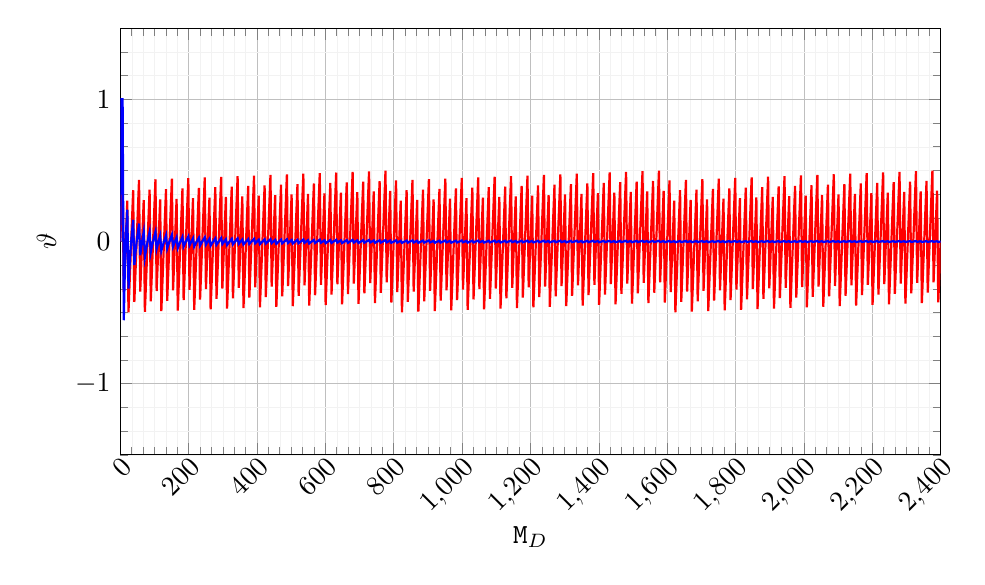
\begin{tikzpicture}
        \begin{axis}[%
            xmin=0,
            xmax=2400,
            ymin=-1.5,
            ymax=1.5,
            samples=700,
            width=12cm,
            height=7cm,
            minor tick num=5,
            grid=both,
            grid style={line width=.1pt, draw=gray!10},
            major grid style={line width=.2pt,draw=gray!50},
            % nodes near coords,
            xlabel near ticks,
            xticklabel style={rotate=45,anchor=north east,inner sep=0mm},
            xlabel={$\texttt{M}_D$},
            ylabel={$\vartheta$},
            ylabel near ticks]
            % \addplot[domain=0:6.4, blue, very thick, smooth, ->] {2.1971*1.8206^x};
            \addplot[domain=0:2400, red, thick] {(x * 0.0625) - round(x / 16)};
            \addplot[domain=0:2400, blue, thick] {((x * 0.0625) - round(x / 16)) / (x * 0.0625)};
        \end{axis}
    \end{tikzpicture}
    \caption[Integerdivisionsinduzierter Rundungsfehler]{Integerdivisionsinduzierter Rundungsfehler der Temperatursensorkonversion
    \textcolor{red}{Rot: Absoluter Fehler $\Delta_{\texttt{M}_D}$.}
    \textcolor{blue}{Blau: Relativer Fehler $\delta_{\texttt{M}_D}$.}
    }
    \label{fig:rounding-err}
\end{figure}
\begin{lstlisting}[language=C]
int temp;
u8 b1, b2;

i2c_smbus_write_byte(test_i2c_client, 0x00);
b1 = i2c_smbus_read_byte(test_i2c_client);
b2 = i2c_smbus_read_byte(test_i2c_client);

temp = (u16)((u16)(b1 << 8) | (u16)(b2));
temp = temp / 16;	// 1 / 0.0625°C = 16

return temp;
\end{lstlisting}

\subsubsection{Potentiometer über \acrshort{spi}}
\subsubsubsection{Protokoll}
\subsubsubsection{Softwareablauf}
\subsubsubsection{Devicetree overlay}
\subsubsection{Fops}
\subsubsection{IOCTL}
\subsubsection{Kompilierung und Verlinkung}
